\documentclass{beamer}
\usepackage{amsmath}
\usepackage{graphicx}
\usepackage{subfigure}

%\usepackage{caption}
%\usepackage{subcaption}

% Copyright 2004 by Till Tantau <tantau@users.sourceforge.net>.
%
% In principle, this file can be redistributed and/or modified under
% the terms of the GNU Public License, version 2.
%
% However, this file is supposed to be a template to be modified
% for your own needs. For this reason, if you use this file as a
% template and not specifically distribute it as part of a another
% package/program, I grant the extra permission to freely copy and
% modify this file as you see fit and even to delete this copyright
% notice. 


\mode<presentation>
{
  \usetheme{default}
  % or ...

  \setbeamercovered{transparent}
  % or whatever (possibly just delete it)
}


\usepackage[english]{babel}
% or whatever

\usepackage[utf8]{inputenc}
% or whatever

\usepackage{xcolor}
\usepackage[percent]{overpic}

\usefonttheme{serif}
\usecolortheme{seahorse}

\usepackage[T1]{fontenc}

\title[April APS]
{Active Resonators for ADMX}

\author[Malagon]
{Ana Malag\'on}

\institute[University of Washington]
{University of Washington, ADMX Collaboration}

\date[April 12, 2015]
{April 15, 2015 / April APS Meeting}

\begin{document}

\begin{frame}
\titlepage
\end{frame}

\begin{frame}{Idea}
\begin{itemize}
\item Axion haloscopes experiments use high-Q microwave cavities.

\item Expected signal power is proportional to Q:
\begin{align*}
P_{sig} \propto \text{min}\big(Q_L, Q_a\big)
\end{align*}
axion quality factor: $Q_a \simeq 10^6$
\item Theoretical Q goes as 
\begin{align*}
Q = \frac{L}{R+L}\frac{R}{\delta}
\end{align*}

\item anomalous skin depth (Cu): $\delta = 2.8\times10^{-5}\text{ cm}\bigg(\frac{\text{GHz}}{f}\bigg)^{1/3}$

\item  $Q_L \approx 10^5$ for $f \approx 1$ GHz.


\item Can we increase the loaded Q further? 
\end{itemize}
\end{frame}

\begin{frame}{Introduce Feedback}
\centering
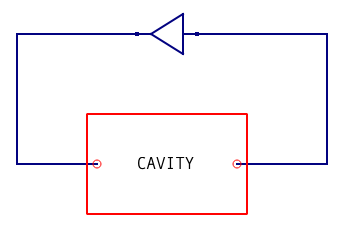
\includegraphics[width=\textwidth]{cavity_linear_to_nonlinear}

\end{frame}

%\begin{frame}{Active Feedback}
%\centering
%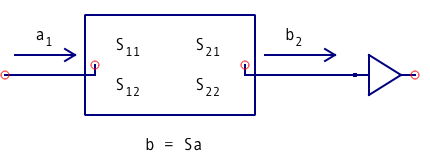
\includegraphics[width=0.6\textwidth]{export_sparams_10}
%\end{frame}
%
%\begin{frame}{Active Feedback}
%\centering
%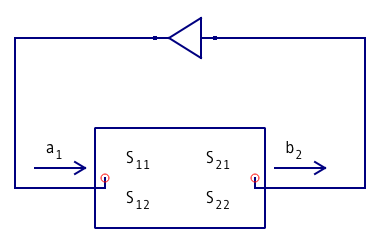
\includegraphics[width=0.65\textwidth]{export_sparams_4}
%\end{frame}

\begin{frame}{Proposal}
\centering
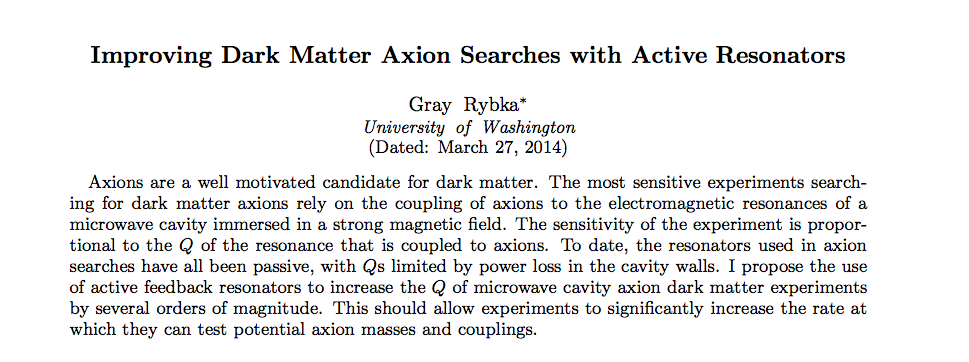
\includegraphics[width=\textwidth]{arxiv_snapshot}

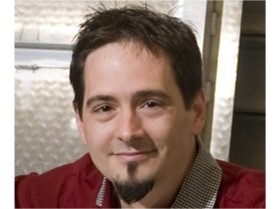
\includegraphics[width=0.3\textwidth]{gray_headshot}
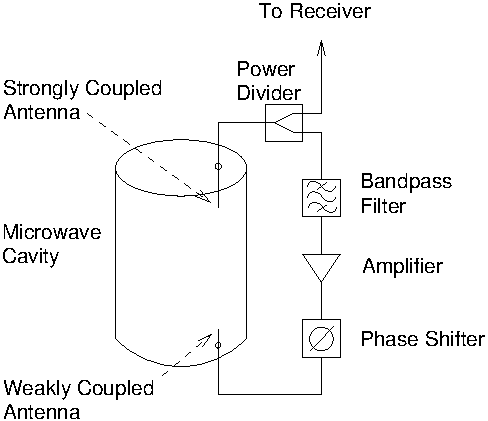
\includegraphics[width=0.3\textwidth]{experiment_schematic-eps-converted-to}

\footnotetext{arXiv:1403.6720}
\end{frame}

\begin{frame}{Active Feedback}
{$V_{out} = V_{in}S_{21}(1 + x + x^2 + \ldots) = V_{in}S_{21}(1-x)^{-1}$}
\begin{columns}
\column{0.65\textwidth}
\centering
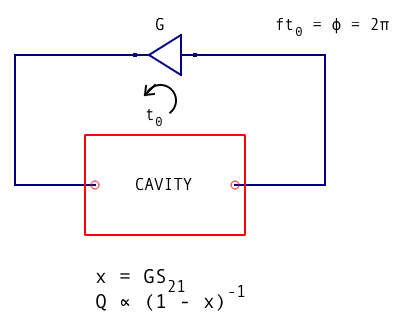
\includegraphics[width=\textwidth]{nonlinear_scaling}
\column{0.35\textwidth}
\begin{itemize}
\item Signal builds up through feedback 
\item Q increases by factor $(1-x)^{-1}$
\item Oscillation begins when $x=1$
\end{itemize}
\end{columns}
\end{frame}

%\begin{frame}{Active Feedback}
%\centering
%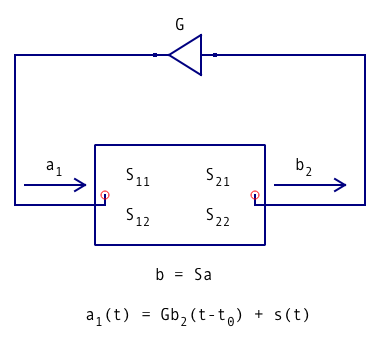
\includegraphics[width=0.65\textwidth]{export_sparams_7}
%\end{frame}
%
%\begin{frame}{Active Feedback}
%\centering
%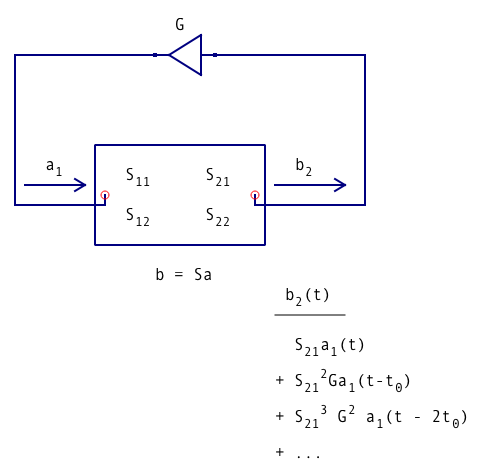
\includegraphics[width=0.65\textwidth]{export_sparams_8}
%\end{frame}
%
%\begin{frame}{Active Feedback}
%\centering
%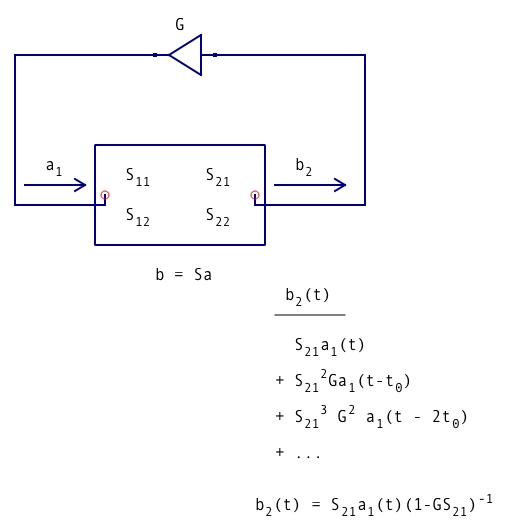
\includegraphics[width=0.65\textwidth]{export_sparams_9}
%\end{frame}
%
%
%\begin{frame}{Active Feedback}
%\centering
%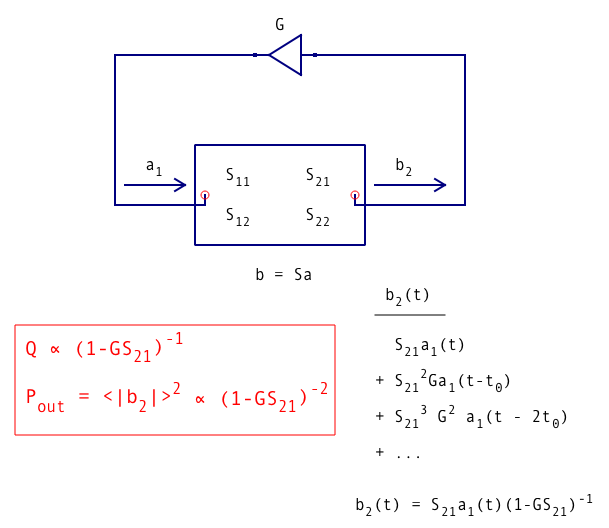
\includegraphics[width=0.65\textwidth]{export_sparams_13}
%\end{frame}
%
%\begin{frame}{Active Feedback}
%\centering
%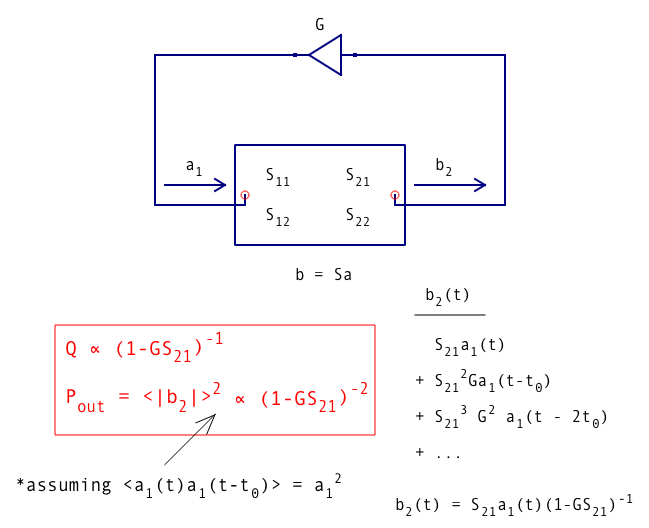
\includegraphics[width=0.65\textwidth]{export_sparams_14}
%\end{frame}

\begin{frame}
\begin{itemize}
\item This idea is old; patented in 1914 and used for making higher gain amplifiers and more selective radio circuits.\footnote{Joe A. Rolf, "Q Multiplier Boosts Selectivity $\&$ Gain," Popular Electronics, April 1974} 

\item However, this amplifies noise and signal equally, so SNR should remain the same for constant amplitude signal:
\begin{align*}
\text{SNR}_{\text{cw}} \propto \text{const.}
\end{align*}
\item Since axion signal is proportional to $Q$, SNR increases
\begin{align*}
\text{SNR}_{\text{axion}} \propto (1-x)^{-1}
\end{align*}
\item We can utilize the different coherence times of signal and noise to get more improvement.
\end{itemize}
\end{frame}

\begin{frame}{Time Delay}
{\tiny Introduce a time delay so $t_0$ greater than cavity coherence time}
\begin{columns}
\column{0.6\textwidth}
\centering
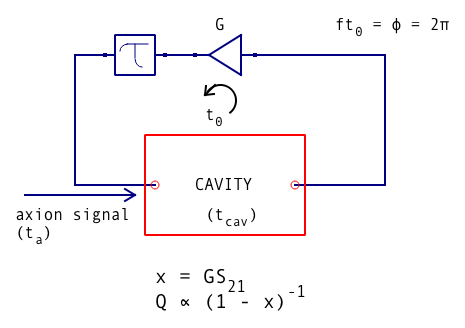
\includegraphics[width=\textwidth]{delay}
\column{0.4\textwidth}
\begin{itemize}
\item Noise is only correlated over time $t_{cav}$
\item Signal is coherent over longer time $t_{a}$
\item If roundtrip time $t_0$ is greater than $t_{cav}$:
\begin{align*}
t_{cav} < t_0 < t_a
\end{align*}
we expect noise to add incoherently and signal
to add coherently

\end{itemize}
\end{columns}
\end{frame}

\begin{frame}{Expected Improvement in Axion SNR}
{\tiny axion snr improvement, $\text{SNR}(x)/\text{SNR}(x=0)$, with and without delay line}
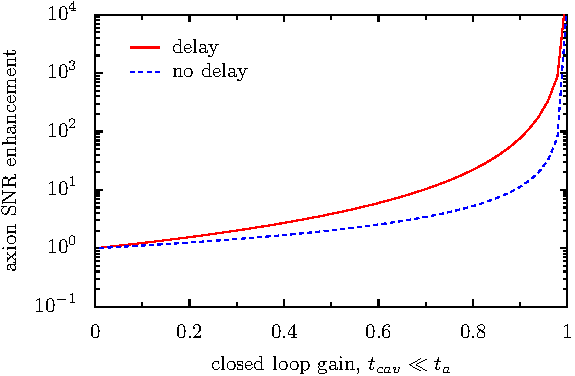
\includegraphics[width=\textwidth]{delay_no_delay}
\end{frame}

\begin{frame}{Expected Improvement in Constant Signal}
{\tiny cw snr improvement, $\text{SNR}(x)/\text{SNR}(x=0)$,  with and without delay line}
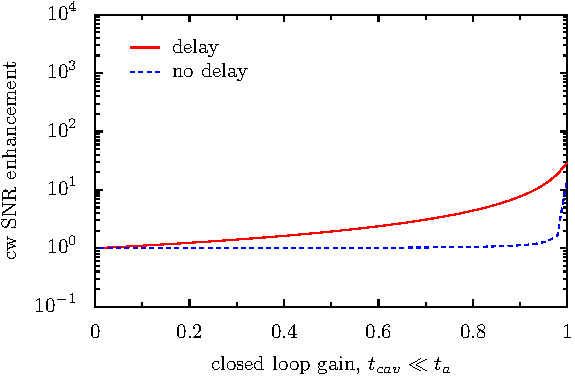
\includegraphics[width=\textwidth]{looking_at_coth}
\end{frame}

\begin{frame}{Initial Setup}
{\tiny feedback using amplifiers, variable attenuator, and phase shifter}
\includegraphics[width=\textwidth]{first_circuit_no_delay}
\end{frame}

\begin{frame}{Q Enhancement}
{\tiny adjusting variable attenuator allows $Q$ to range from 1000 to 9000 before oscillations begin}
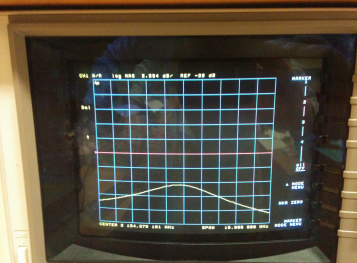
\includegraphics[width=0.5\textwidth]{low_q}
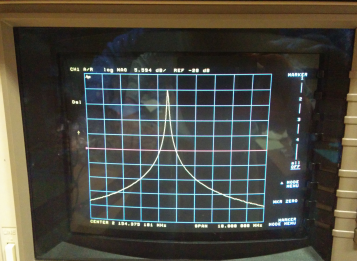
\includegraphics[width=0.5\textwidth]{high_q}
\end{frame}

\begin{frame}{Setup}
\includegraphics[width=\textwidth]{first_circuit_version}
\end{frame}

%\begin{frame}{Active Feedback Resonator}
%{\tiny Ouroboros}
%%\begin{columns}
%%\column{0.5\textwidth}
%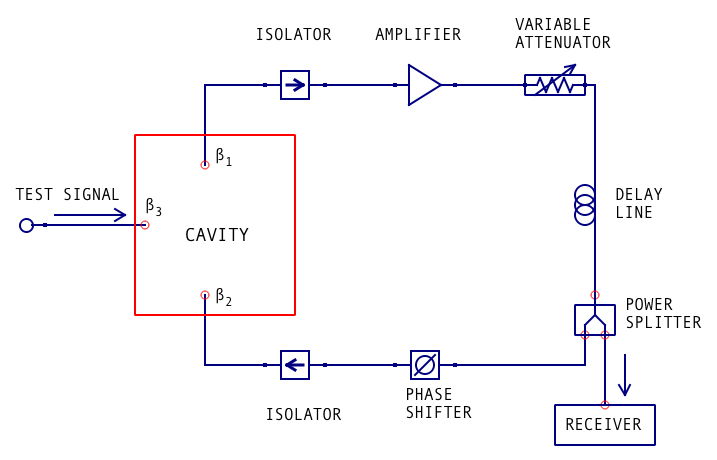
\includegraphics[width=\textwidth]{export_ouroboros}
%%\column{0.5\textwidth}
%%\begin{itemize}
%%\item $t$: time around loop
%%\item $\tau$: coherence time of cavity
%%\item Intuition: signal feeds back coherently; when $t > \tau$, noise adds incoherently
%%\end{itemize}
%%\end{columns}
%\end{frame}

\begin{frame}{Schematic}
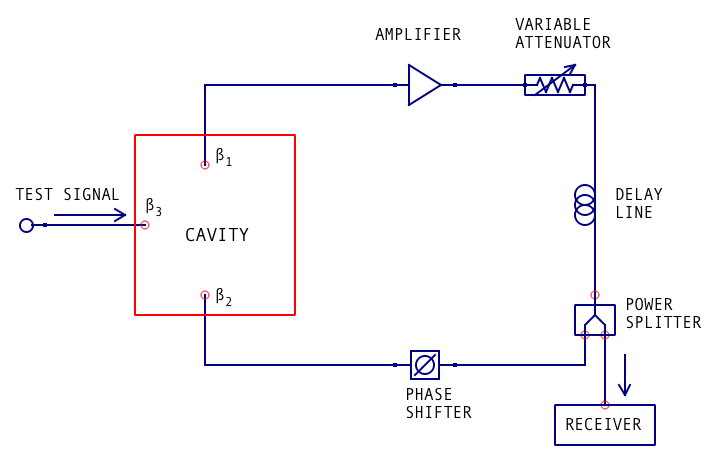
\includegraphics[width=\textwidth]{no_isolator}
\end{frame}


\begin{frame}{Parameters}
\begin{columns}
\column{0.5\textwidth}
\begin{tabular}{| l l |}
\hline
Parameter & Values \\
\hline
\hline
$f_{\text{cav}}$ & 2.256 GHz \\ 
$t_{\text{delay}}$ & 2.4 $\mu$s \\
$t_{\text{cav}}$ & 170 ns \\ 
$t_{\text{axion}}$ & 141 $\mu$s \\
\hline
\end{tabular}
\column{0.5\textwidth}
Experiment
\begin{itemize}
\item Set attenuation of variable attenuator
\item Adjust phase so Q is maximal
\item Measure Q, $f_{cav}$
\item Inject constant amplitude signal at $f_{cav}$
\item Measure height of signal relative to noise floor in detected spectrum
\end{itemize}
\end{columns}
\end{frame}

%\begin{frame}{Axion and CW Signal}
%{\tiny Scenario 1}
%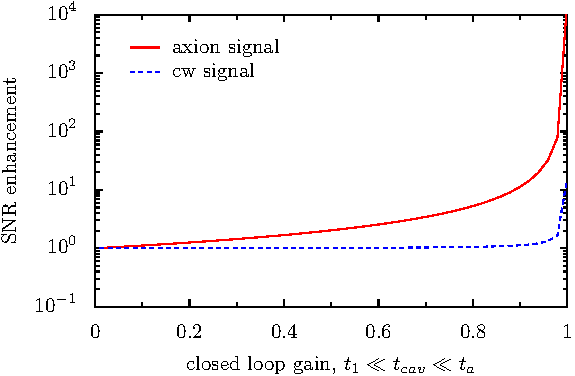
\includegraphics[width=\textwidth]{first_limit}
%
%\end{frame}
%
%\begin{frame}{Axion and CW Signal}
%{\tiny Scenario 2}
%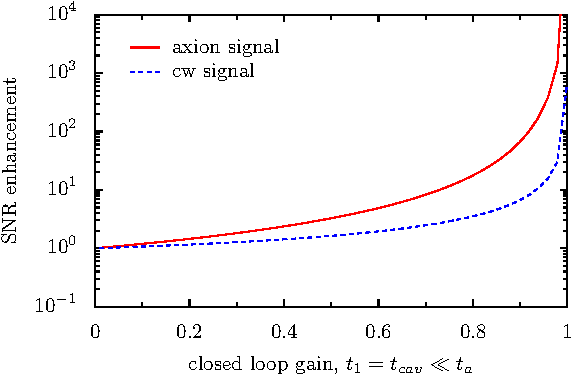
\includegraphics[width=\textwidth]{second_limit}
%\end{frame}
%
%\begin{frame}{Axion and CW Signal}
%{\tiny Scenario 3}
%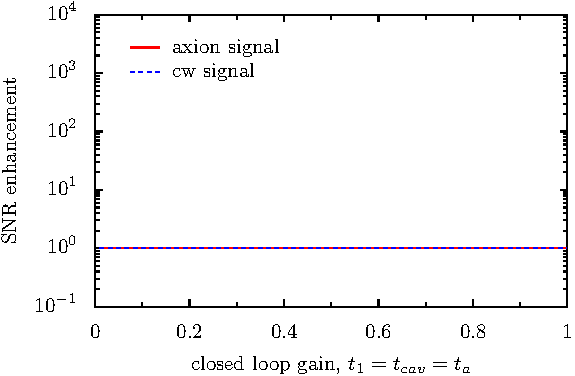
\includegraphics[width=\textwidth]{third_limit}
%\end{frame}


%\begin{frame}{Exploring Second Limit}
%{\tiny$t_1 \ll t_{cav}$}
%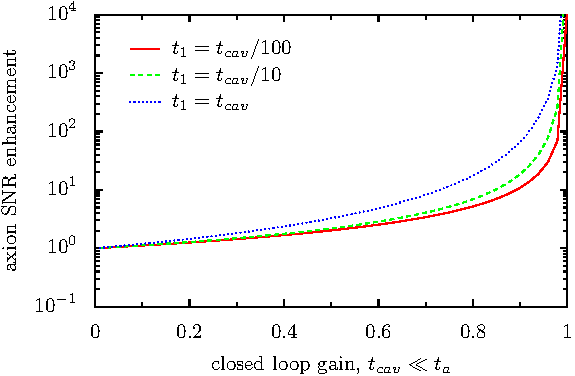
\includegraphics[width=\textwidth]{exploring_second_limit_low}
%\end{frame}
%
%\begin{frame}{Exploring Second Limit}
%{\tiny $t_1 > t_{cav}$}
%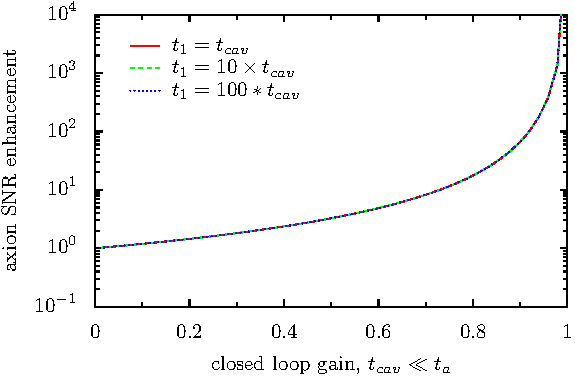
\includegraphics[width=\textwidth]{exploring_second_limit_high}
%\end{frame}

%\begin{frame}{Theory and Experiment}
%{Comparison}
%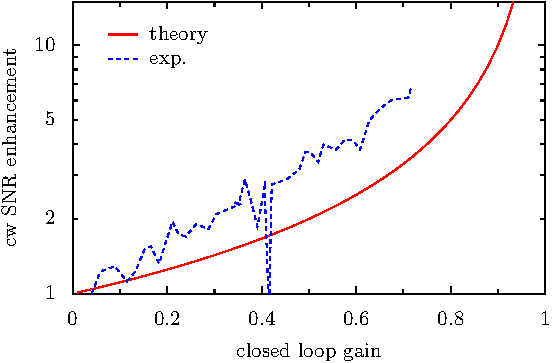
\includegraphics[width=\textwidth]{comparison_xaxis_gain}
%\end{frame}


%\begin{frame}{Active Feedback Resonator}
%{\tiny Ouroboros}
%\begin{columns}
%\column{0.5\textwidth}
%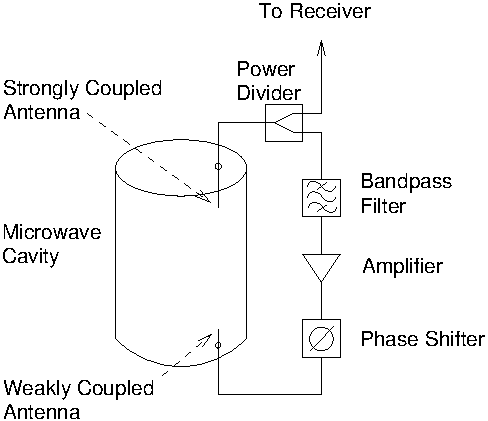
\includegraphics[width=\textwidth]{experiment_schematic-eps-converted-to}
%\column{0.5\textwidth}
%\begin{itemize}
%\item $t$: time around loop
%\item $\tau$: coherence time of cavity
%\item Intuition: signal feeds back coherently; when $t > \tau$, noise adds incoherently
%\end{itemize}
%\end{columns}
%\end{frame}

%\begin{frame}{Equivalent Circuit}
%\centering
%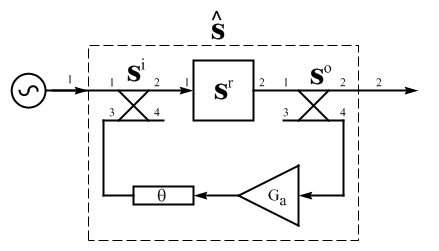
\includegraphics[width=.5\textwidth]{qmultiplier}
%
%$G_l$ the loop gain\\
%$Q_0$ the active quality factor\\
%$T_a$ the amplifier noise temperature\\
%%$T_{cav}$ the cavity noise temperature\\
%\begin{columns}
%\column{0.5\textwidth}
%\centering
%\begin{align*}
%Q_0 = Q_L(1-\sqrt{G_l})^{-1} \\
%|\hat{S}_{21}|^2 \propto (1- \sqrt{G_l})^{-2}
%\end{align*}
%\column{0.5\textwidth}
%\centering
%\begin{align*}
%T_{noise} = \frac{T_{cav} + G_l T_a}{1 + G_l - 2\sqrt{G_l}e^{-t/\tau - i\theta}}
%\end{align*}
%\end{columns}
%\end{frame}

%\begin{frame}{Prototype}
%\begin{columns}
%\column{0.5\textwidth}
%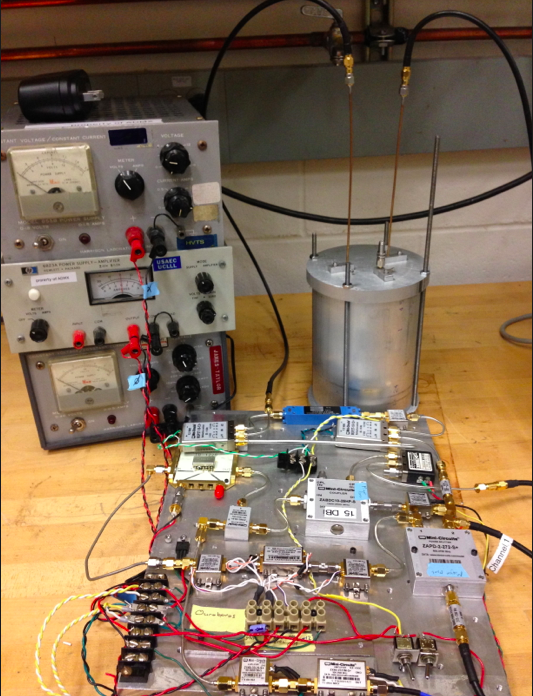
\includegraphics[width=\textwidth]{active_resonator_setup_photo}
%\column{0.5\textwidth}
%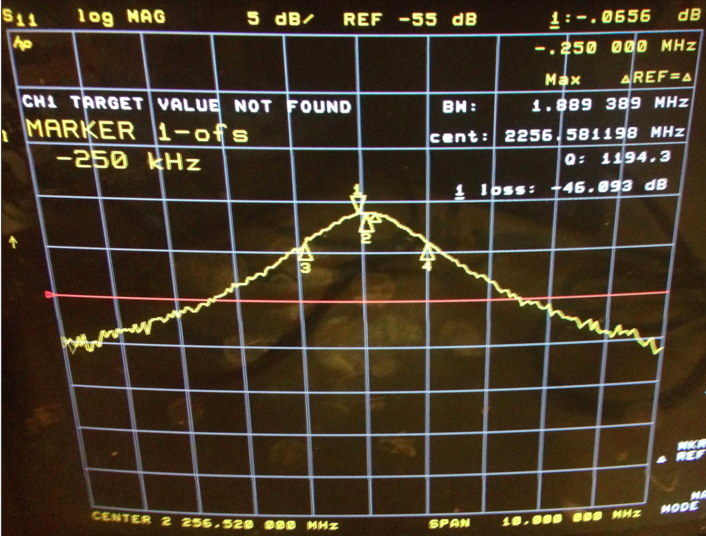
\includegraphics[width=\textwidth]{s21_no_delay}
%
%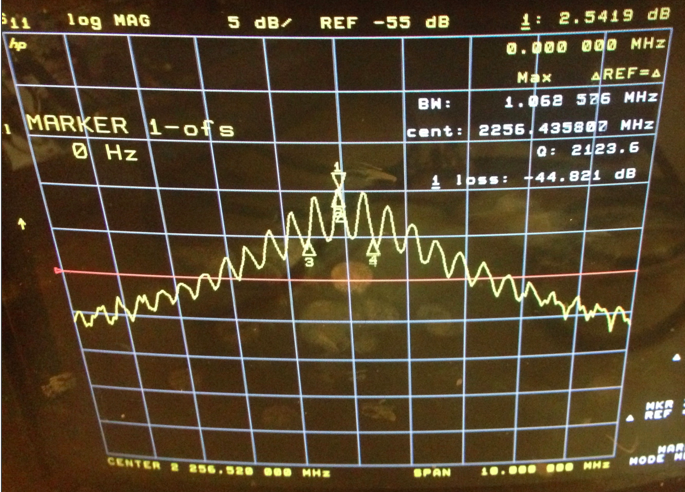
\includegraphics[width=\textwidth]{s21_delay}
%\end{columns}
%
%\end{frame}

\begin{frame}{Results}
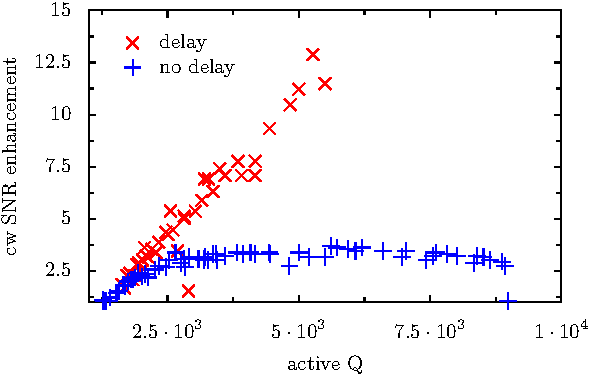
\includegraphics[width=\textwidth]{experiment}
\end{frame}

\begin{frame}{Considerations}
\begin{itemize}
\item move to digital delay lines
\item major design considerations would center around gain instability; to get $10$x increase in Q, need $x \simeq 0.9$.
\end{itemize}
\end{frame}

\begin{frame}{Conclusions}
\begin{itemize}
\item active feedback is a simple technique to increase Q
\item delay line provides additional increase in SNR
\item independent of other parts of the experiment
\item does not need to be operated cryogenically
%\item phase shifter allows for fine tuning of resonance
\end{itemize}
\end{frame}


\begin{frame}{People}
{Lisa McBride, Kunal Patel, Gray Rybka}
{\tiny This work was supported by the Dept. of Energy, Division of High Energy Physics.}

\begin{columns}
\column{0.5\textwidth}
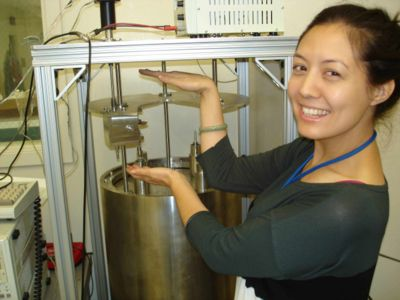
\includegraphics[width=0.8\textwidth]{lisa_pic}
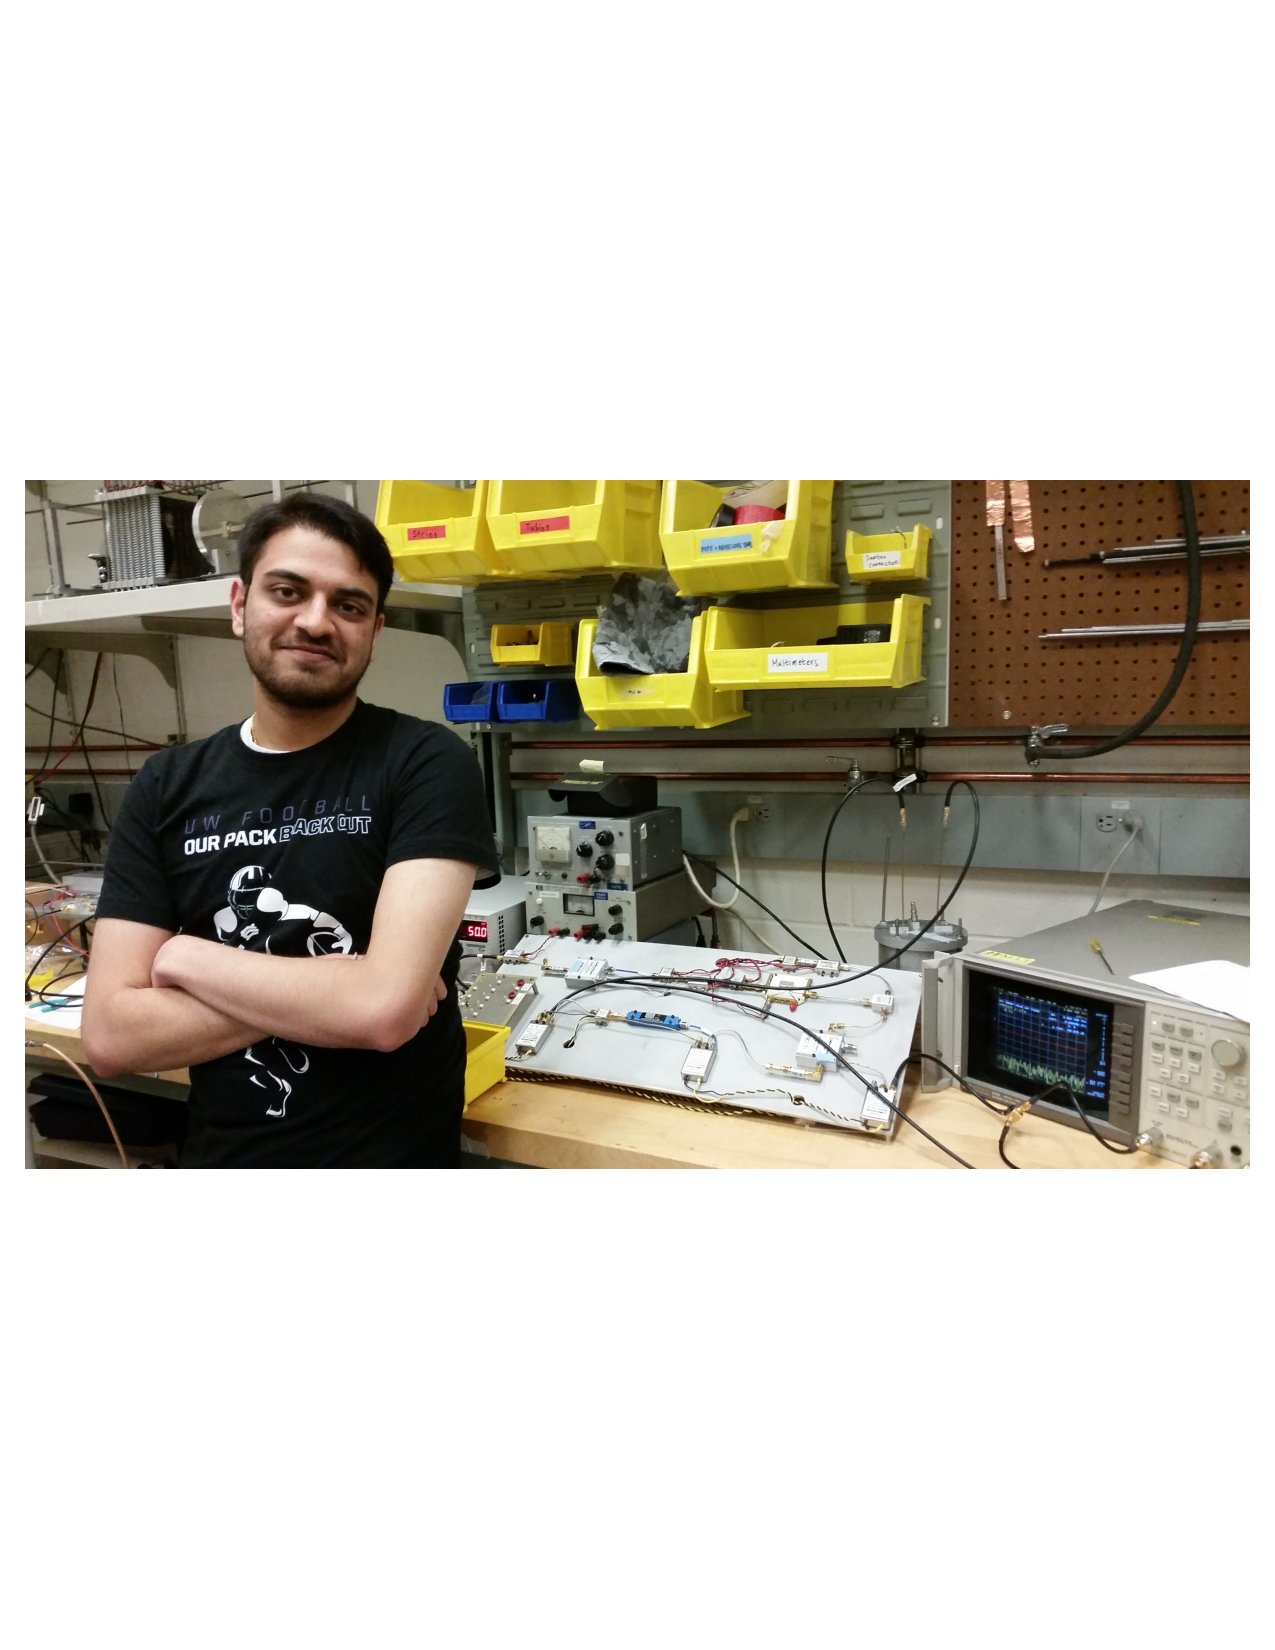
\includegraphics[width=\textwidth]{kunal_pic}

\column{0.5\textwidth}
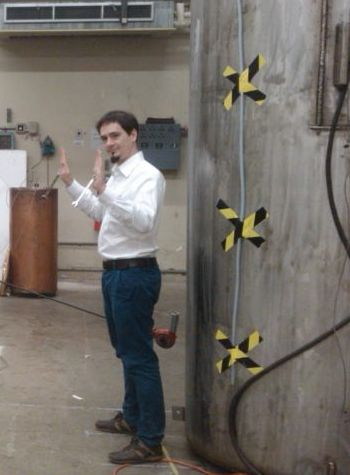
\includegraphics[width=\textwidth]{gray_pic}

\end{columns}

\end{frame}

%\begin{frame}{Acknowledgments}
%DOE HEP
%\end{frame}





\begin{frame}{Backup}
\centering
Backup Slides
\end{frame}

\begin{frame}{If $Q_L > Q_a$}
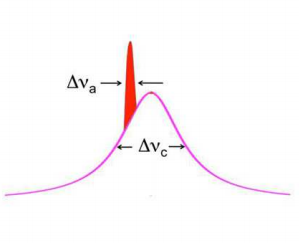
\includegraphics[width=0.5\textwidth]{axion_bw}

If cavity Q is larger than axion Q (or $t_{cav} > t_a$), we no longer detect the full axion power within the cavity bandwidth.
\end{frame}

\begin{frame}{Delay Lines}
{\tiny Surface Acoustic Wave (SAW) Resonator}
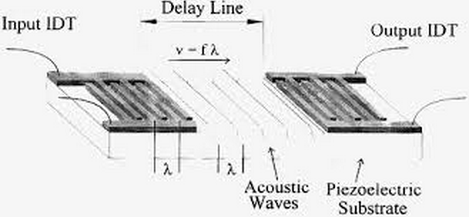
\includegraphics[width=\textwidth]{saw}
\end{frame}

\begin{frame}{Expected SNR Improvement}
{\tiny analysis of signal correlation}
Scenario 1: $t_0 \ll t_{cav}$: .
\begin{align*}
\langle V_{in}(t)V_{in}(t-t_0)\rangle &= \bar{V}_{in}^2\\
\langle|V_{out}|^2\rangle = |\bar{V}_{in}S_{21}|^2(1 + x + x^2 + \ldots)^2 &= \bar{V}_{in}^2|S_{21}|^2(1-x)^{-2}
\end{align*}
Scenario 2: $t_0 \sim \mathcal{O}(t_{cav})$:  
\begin{align*}
\langle V_{in}(t)V_{in}(t-t_0)\rangle &= \bar{V}_{in}^2e^{-t_0/t_{cav}}\\
\langle|V_{out}|^2\rangle &=  |\bar{V}_{in}S_{21}|^2(1 + xe^{-t_0/t_{cav}} + x^2e^{-2t_0/t_{cav}} + \ldots)^2 \\
&= \bar{V}_{in}^2|S_{21}|^2(1-xe^{-t_0/t_{cav}})^{-2}
\end{align*}
this analysis is not completely correct - it predicts a turnover at x=0.5. One needs to treat the nonlinearity properly to get the correct result:
\begin{align*}
\langle|V_{out}|^2\rangle = \frac{\bar{V}_{in}^2|S_{21}|^2}{(1-x)^{2}}\frac{1 + xe^{-t_0/t_{cav}}}{1 - xe^{-t_0/t_{cav}}}
\end{align*}
\end{frame}

\begin{frame}{Comparison (preliminary)}
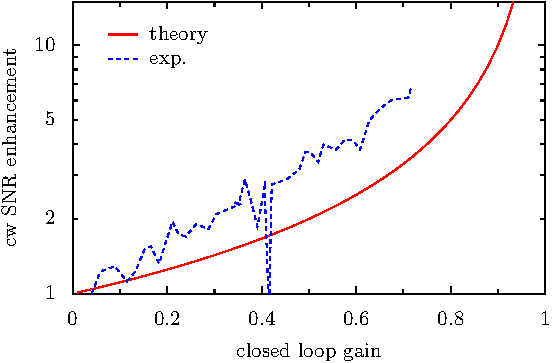
\includegraphics[width=\textwidth]{comparison_xaxis_gain}
\end{frame}

\begin{frame}{Interference Fringes}
When $\Delta f t_0 > \pi$, one sees interference fringes, due to off resonant signals acquiring an extra phase shift of $\pi/2$ relative to the phase acquired by the resonant frequency.
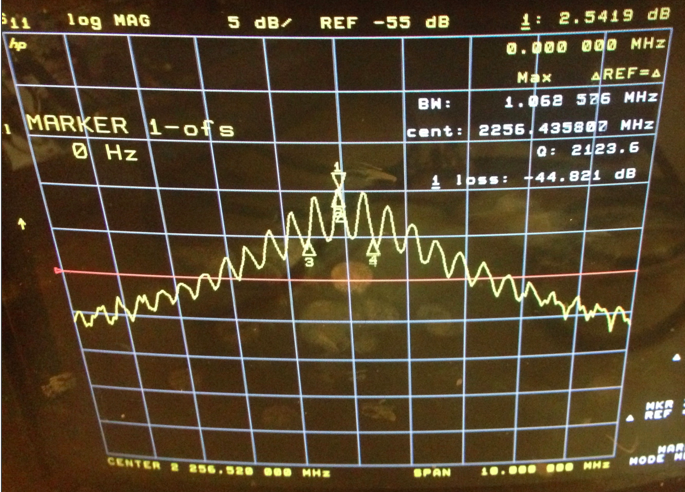
\includegraphics[width=\textwidth]{s21_delay}
\end{frame}

\end{document}